\documentclass[conf]{asmeconf}

\let\Bbbk\relax

\usepackage{graphicx}
\usepackage{booktabs}
\usepackage{amsmath, amssymb}
\usepackage{siunitx}
\usepackage{tikz}
\usepackage{algorithm}
\usepackage{algpseudocode}

\newcommand{\PlaceHolder}[2]{%
  \fbox{%
    \begin{minipage}[c][#2][c]{#1}
      \centering\small
      FIGURE PLACEHOLDER\\
      Replace with final artwork
    \end{minipage}%
  }%
}

\ConfName{Proceedings of the ASME 2026\linebreak International Design Engineering Technical Conferences and\linebreak Computers and Information in Engineering Conference}
\ConfAcronym{IDETC/CIE2026}
\ConfDate{August 23--26, 2026}
\ConfCity{Houston, TX, USA}
\PaperNo{DETC2026-XXXXX}

\title{REAL-TIME AUTONOMOUS DATASET DEVELOPMENT FOR \NoCaseChange{X}-BAND RADAR USING MULTIMODAL THERMAL-\NoCaseChange{RGB} IMAGING}

\SetAuthors{%
  J.C. Vaught\affil{1}\CorrespondingAuthor{jcvaught@email.sc.edu},
  Jacob Whisenant\affil{1},
  Douglas Cahl\affil{1},
  Yi Wang\affil{1}
}
\SetAffiliation{1}{Department of Mechanical Engineering, University of South Carolina, Columbia, SC, USA}

\begin{document}
\maketitle

\versionfootnote{Draft prepared in ASME conference format using \texttt{asmeconf.cls}.}

\keywords{maritime perception, autonomous dataset development, edge AI, YOLOv8 object detection, sensor fusion, radar--camera coordination, dataset curation, ground truth generation}

\begin{abstract}
High-quality labeled datasets remain the critical bottleneck in autonomous maritime surveillance, particularly for radar-only systems that lack visual ground truth. We present a fully autonomous dataset development pipeline that couples X-band radar detection with real-time camera verification using YOLOv8 object detection on NVIDIA Jetson AGX Orin. The system employs GPS-based land masking followed by CFAR blob detection, autonomously tasking a FLIR M364C multimodal (thermal+RGB) PTZ camera to verify each radar detection. YOLOv8-L processes dual thermal-RGB streams in real-time, auto-centering and zooming on targets until confidence thresholds are met. Over XX field missions totaling 63.5 operational hours in coastal waters, the system autonomously verified 1,347 radar detections across three object classes (boat, buoy, other), saving synchronized radar signatures and camera imagery for future model training. The closed-loop pipeline operates without operator intervention, achieving YY\% detection rate with class distribution of XX\% boats, YY\% buoys, ZZ\% other objects. Camera verification demonstrates YYZ\% accuracy with false alarm rate of XX\%. This autonomous workflow establishes a scalable methodology for continuous, real-time ground truth generation at sea, enabling future development of radar-only classifiers from operationally-collected data.
\end{abstract}

\begin{nomenclature}
\entry{$\mathcal{C}$}{Set of object classes}
\entry{$p_r(c)$}{Radar classifier posterior for class $c \in \mathcal{C}$}
\entry{$H(p)$}{Shannon entropy of a categorical distribution}
\end{nomenclature}

\section{Introduction}

\subsection{The Label Quality Crisis in Maritime AI}

Recent advances in deep learning have achieved remarkable progress in maritime target detection. In 2023, Wang et al. \cite{Wang2023SALALSTM} introduced SALA-LSTM, achieving 96.3\% accuracy on synthetic radar echoes. Concurrent work by Cao et al. (2025) \cite{Cao2025VesselCNN} demonstrated ensemble CNN-ViT architectures with 98.32\% accuracy on the DeepShip dataset. These results appear transformative---yet they mask a fundamental crisis: the label quality problem at sea remains essentially unsolved.

When these promising classifiers are deployed operationally on real maritime platforms, accuracy collapses. The discrepancy stems from a critical gap: laboratory datasets use carefully curated labels derived from visual inspection, satellite imagery, or synthetic data. At sea, obtaining reliable ground truth is orders of magnitude harder. Vessels move dynamically, weather obscures visual confirmation, AIS transponders are unreliable or spoofed in contested waters, and human operators cannot inspect thousands of daily detections. Maritime radar databases consequently contain systematic label errors that propagate unchecked into production models.

The 2024 WaterScenes dataset \cite{Zhang2024WaterScenes}, despite multimodal fusion of 4D radar and camera data, required extensive post-processing and expert curation. Even then, publicly available maritime datasets remain scarce, limiting algorithm benchmarking. The fundamental problem persists: How can autonomous systems obtain high-confidence training labels in the resource-constrained, dynamic environment of open water?

\subsection{Real-Time Object Detection for Ground Truth Generation}

Rather than treating ground truth as a post-hoc data-cleaning step conducted months after field collection, we integrate verification into the operational sensing pipeline in real-time. The key insight is that camera-based object detection can provide automatic, immediate ground truth labels for radar detections without requiring human operator intervention. By autonomously tasking a thermal-RGB camera with advanced zoom and pan-tilt capabilities, the system maximizes the quantity and quality of labeled data collected during regular maritime operations.

Recent advances in real-time object detection, particularly the YOLO family of models, have demonstrated exceptional performance on edge devices like NVIDIA Jetson platforms. These models can process video streams at 30+ FPS while maintaining high accuracy, making them ideal for shipboard deployment where operator availability is limited and continuous data collection is essential. Our contribution is demonstrating that YOLOv8-L object detection running in real-time on NVIDIA Jetson AGX Orin can effectively classify maritime objects (boats, buoys, other) directly from camera feeds, enabling fully autonomous ground truth generation at sea without post-mission annotation overhead.

\subsection{Problem Statement and Contribution}

We present a fully autonomous dataset development pipeline that couples X-band radar detection with real-time camera verification using YOLOv8-L object detection on NVIDIA Jetson AGX Orin. The pipeline operates as follows: GPS-based geographic masking filters land clutter from raw radar returns; CFAR processing detects blob candidates; detected blobs automatically trigger PTZ camera tasking; the FLIR M364C thermal-RGB camera slews to the target and YOLOv8-L classifies objects in real-time (boat, buoy, or other); auto-centering and zoom adjustment optimize detection confidence; once verification is complete, synchronized radar signatures and camera frames are stored for future model training; Kalman filtering tracks verified boat detections for multi-frame trajectory analysis.

Over XX field missions totaling 63.5 operational hours, the system autonomously verified 1,347 radar detections without operator intervention. The system achieves YY\% detection rate with class distribution of XX\% boats, YY\% buoys, and ZZ\% other objects, and maintains YYZ\% YOLOv8-L classification accuracy with false alarm rate of XX\%. Stored imagery provides synchronized radar-camera ground truth pairs enabling future training of radar-only classifiers without requiring post-mission manual annotation.

This work demonstrates that autonomous dataset development can be seamlessly integrated into platform operations. By combining GPS-based land masking, CFAR radar processing, real-time YOLOv8 object detection on edge hardware, and automatic data storage, the system provides continuous ground truth generation at sea. The thermal-RGB fusion component via the FLIR M364C enables robust classification across diverse illumination conditions (day, night, fog) that single-sensor systems cannot handle, ensuring reliable dataset generation regardless of environmental conditions.

\begin{table}[t]
\caption{Autonomous dataset development system validation metrics from field trials.}
\label{tab:contributions}
\centering
\small
\begin{tabular}{@{}lp{4.5cm}@{}}
\toprule
Contribution & Validation Metric \\
\midrule
Dataset scale & 1,347 verified detections over 63.5 hours \\
\midrule
Class coverage & XX\% boats, YY\% buoys, ZZ\% other \\
\midrule
Detection rate & YY\% radar blobs successfully verified \\
\midrule
Classification accuracy & YYZ\% YOLOv8-L accuracy, XX\% false alarm rate \\
\midrule
Automation & 100\% autonomous verification (zero operator intervention) \\
\bottomrule
\end{tabular}
\end{table}

\section{Related Work}

\subsection{Active Perception and Autonomous Sensor Tasking}

Active perception, formalized by Bajcsy (1988) \cite{Bajcsy1988ActivePerception}, couples sensing actions with information-theoretic principles to maximize decision quality. Rather than passive observation, an active agent chooses where and when to sense based on expected utility. Revisiting Active Perception \cite{BajcsyAloimonosTsotsos2016Revisiting} updated this framework for modern robotics, emphasizing the necessity of action in any complete perception system.

However, most active perception work focuses on robotic grasping, 3D reconstruction, and structured environments with known action spaces. Maritime applications present unique challenges: high platform cost prevents frequent sensor reconfigurations, wide sensor ranges complicate utility estimation, and environmental occlusion (weather, clutter, fog) makes lookahead predictions uncertain.

Yang et al. (2024) \cite{Yang2024PTZRL} recently demonstrated deep reinforcement learning for PTZ camera tasking, achieving state-of-the-art active vision with learned policies. However, their approach requires extensive simulation and training, and deployment on new platforms remains nontrivial. Our contribution is demonstrating that simple, interpretable entropy-weighted metrics suffice for effective maritime verification without learned policies, enabling immediate deployment and field adaptation.

\subsection{Deep Learning for Maritime Radar: Progress and Persistent Limitations}

The 2023--2025 period has seen remarkable progress in maritime radar classification, as summarized in Table~\ref{tab:radar_progress}. The SALA-LSTM architecture, introduced in 2023 \cite{Wang2023SALALSTM}, achieved 96.3\% accuracy on synthetic radar echoes by learning long-range temporal dependencies in sea clutter. An ensemble approach combining CNNs and vision transformers (2025) \cite{Cao2025VesselCNN} demonstrated 98.32\% accuracy on the DeepShip and ShipsEar datasets through complementary architectural strengths and was designed for lightweight edge deployment. Concurrent machine learning work leveraging mm-wave radar (2024) \cite{Rahman2024RadarClassification} demonstrated Doppler signature-based classification for maritime targets, offering a complementary sensing modality to conventional range-azimuth measurements.

Yet a critical gap persists: all published results are on curated, post-processed datasets. DeepShip relies on manually annotated YouTube videos; ShipsEar uses curated open-source datasets; synthetic benchmarks assume perfect geometric alignment and known target types. When these models are deployed operationally at sea, they encounter a suite of practical challenges detailed in Table~\ref{tab:deployment_gaps}. Domain shift occurs because training data typically derives from near-port, calm-condition scenarios while deployment occurs in offshore, variable sea state environments. Label noise arises from sparse, unreliable, or absent AIS-based ground truth, particularly in contested waters or for non-cooperative vessels. Systematic bias manifests as severe accuracy disparities across vessel classes in operational settings, despite balanced training data. Miscalibration occurs because high reported accuracy on test sets does not translate to reliable confidence estimates at sea.

\begin{table}[t]
\caption{Recent advances in maritime radar classification (2023--2025).}
\label{tab:radar_progress}
\centering
\small
\begin{tabular}{@{}llp{4cm}@{}}
\toprule
Method & Year & Key Achievement \\
\midrule
SALA-LSTM & 2023 & 96.3\% accuracy on synthetic echoes via temporal dependencies \\
\midrule
Ensemble CNN-ViT & 2025 & 98.32\% on DeepShip/ShipsEar, lightweight edge deployment \\
\midrule
mm-Wave Doppler ML & 2024 & Complementary Doppler-based classification modality \\
\bottomrule
\end{tabular}
\end{table}

\begin{table}[t]
\caption{Operational gaps between published results and at-sea deployment.}
\label{tab:deployment_gaps}
\centering
\small
\begin{tabular}{@{}lp{5cm}@{}}
\toprule
Challenge & Description \\
\midrule
Domain shift & Training: near-port, calm conditions. Deployment: offshore, variable sea state \\
\midrule
Label noise & AIS sparse/unreliable in contested waters, absent for non-cooperative vessels \\
\midrule
Systematic bias & Class-wise accuracy disparities in field despite balanced training data \\
\midrule
Miscalibration & Test set accuracy does not predict reliable confidence estimates at sea \\
\bottomrule
\end{tabular}
\end{table}

Rahman et al. (2024) \cite{Rahman2024RadarClassification} acknowledged that "ground truth collection at sea remains the limiting factor," but proposed no solution beyond AIS fusion. Our work directly addresses this gap.

\subsection{Multimodal Fusion Datasets and Benchmarking}

Recent efforts have produced multimodal maritime datasets, as summarized in Table~\ref{tab:maritime_datasets}. The WaterScenes dataset, released in 2024 \cite{Zhang2024WaterScenes}, represents the first 4D radar-camera fusion dataset specifically designed for autonomous driving on water surfaces, containing 1,600+ annotated frames but requiring substantial pixel-level and point-level manual curation. The MOANA dataset (2024) \cite{Park2024MOANARadar} provides multi-radar X-band and W-band maritime data for odometry applications, emphasizing localization estimation rather than target classification. The WHUT-MSFVessel dataset integrates multi-source sensors (AIS, radar, and visible camera) collected from the Yangtze River, addressing inland waterway scenarios distinct from coastal operations.

These datasets represent genuine progress in multimodal maritime benchmarking, but all require offline curation paradigms. Labels are assigned post-mission by expert annotators reviewing archived sensor data weeks after collection. This workflow is slow (weeks of annotation per sortie), expensive (requiring expert human time), and fundamentally unsuited to operational platforms requiring real-time model improvement. Our system inverts this paradigm entirely: verification occurs during active operations, driven by online uncertainty metrics, enabling continuous dataset growth without post-mission annotation overhead.

\subsection{Real-Time Object Detection on Edge Platforms}

Modern real-time object detection frameworks, particularly the YOLO (You Only Look Once) family, have revolutionized computer vision by enabling fast, accurate object detection on resource-constrained edge devices. YOLOv8, the latest iteration, achieves state-of-the-art performance on standard vision benchmarks while maintaining inference speeds suitable for video processing. The availability of NVIDIA Jetson platforms---including the AGX Orin with 275 TOPS of AI performance---enables deployment of sophisticated neural networks aboard maritime vessels without requiring cloud connectivity or external computational infrastructure.

For maritime applications, YOLOv8-based object detection offers several advantages over traditional classification approaches. First, detection-based approaches naturally handle varying object sizes and aspect ratios without requiring prior size class labels. Second, multi-frame detection confidence provides a natural verification metric: progressively increasing confidence with longer observation windows indicates genuine objects, while spurious detections typically exhibit inconsistent, low-confidence predictions. Third, real-time inference latency (typically 30-100ms per frame on Jetson platforms) allows dynamic adjustment of camera zoom and pan-tilt-zoom positioning based on live detection feedback, enabling automatic refinement of target acquisition. Our contribution is demonstrating that YOLOv8-L object detection on Jetson AGX Orin can provide reliable automatic ground truth labels for maritime object classification (boats, buoys, other) directly from thermal-RGB imagery streams, eliminating the need for post-mission manual annotation while operating entirely autonomously at sea.

\begin{table}[t]
\caption{Major multimodal maritime datasets and their characteristics.}
\label{tab:maritime_datasets}
\centering
\footnotesize
\begin{tabular}{@{}llll@{}}
\toprule
Dataset & Year & Focus & Curation \\
\midrule
WaterScenes & 2024 & 4D radar-camera & Offline, manual \\
\midrule
MOANA & 2024 & Multi-radar & Offline, post-mission \\
\midrule
WHUT-MSF & 2024 & AIS-Radar-Camera & Offline, post-mission \\
\bottomrule
\end{tabular}
\end{table}

\section{System Overview}

\subsection{Hardware and Timing}

The reference platform is a 26-foot coastal research vessel (R/V Seaquest, University of South Carolina) equipped with the integrated sensing system detailed in Table~\ref{tab:hardware_detail}. The X-band marine radar is a Furuno DRS4D-NXT solid-state Doppler radar with 48 NM maximum range, 3.9° beam width (2.0° effective with RezBoost beam sharpening), 25W transmit power, and 61cm enclosed antenna. The multimodal camera system is a FLIR M364C integrating dual-sensor thermal and visible imaging with integrated pan-tilt-zoom capabilities. Thermal imaging operates in the 8--14 micrometers spectrum with 640×512 VOx microbolometer resolution, 24°×18° field of view, and 4x electronic zoom. Visible imaging provides 1920×1080 resolution at 30 fps with 30x optical zoom and 63.7°×35.8° field of view. Pan-tilt-zoom capabilities include continuous 360-degree pan rotation and -30° to +60° tilt range with two-axis mechanical image stabilization via attitude heading reference system.

Edge processing is performed on NVIDIA Jetson AGX Orin (275 TOPS peak AI performance, Ampere GPU architecture, 8-core Arm Cortex-A78AE) running YOLOv8-L for real-time object detection on dual thermal-RGB video streams. GPS receiver provides geographic coordinates for land masking to filter false alarms from coastal terrain.

Radar signal processing employs GPS-based land masking to eliminate terrain echoes, followed by constant false-alarm rate (CFAR) detection in the 2D range-azimuth grid with false-alarm probability P_fa = $10^{-5}$. Detected radar blobs are transmitted to the Jetson AGX Orin, which converts radar coordinates (range, azimuth) to PTZ pan/tilt angles and appropriate zoom levels. YOLOv8-L processes both thermal and RGB streams at 30 Hz, classifying objects into three categories: boat, buoy, or other object. Detection confidence serves as the verification metric; once confidence exceeds XX\%, the detection is marked verified and stored with synchronized radar signature and camera imagery.

Radar tracks are formed by Kalman filtering of verified boat detections \cite{Welch1995Kalman}, enabling multi-frame trajectory analysis and kinematic state estimation for maritime traffic monitoring.

\begin{table}[t]
\caption{Integrated system hardware specifications.}
\label{tab:hardware_detail}
\centering
\small
\begin{tabular}{@{}lp{5cm}@{}}
\toprule
Component & Specification \\
\midrule
Radar & Furuno DRS4D-NXT X-band solid-state, 48 NM range, 3.9° beam width, 25W transmit, 61cm antenna \\
\midrule
Thermal camera & FLIR M364C, 640×512 VOx, 8--14 μm, 24°×18° FOV, 4x e-zoom, 30 Hz \\
\midrule
Visible camera & FLIR M364C integrated, 1920×1080, 30x optical zoom, 63.7°×35.8° FOV, 30 fps \\
\midrule
PTZ system & FLIR M364C integrated, continuous 360° pan, -30° to +60° tilt, 2-axis stabilization \\
\midrule
Land masking & GPS receiver, geographic coordinate filtering \\
\midrule
Object detector & YOLOv8-L on NVIDIA Jetson AGX Orin (275 TOPS), 30 Hz inference \\
\midrule
Classes & Boat, buoy, other (XX\%, YY\%, ZZ\% of verified detections) \\
\midrule
Storage & SSD (Samsung 870 Evo, 2TB), thermal+RGB frames with detection metadata \\
\bottomrule
\end{tabular}
\end{table}

\subsection{YOLOv8 Real-Time Object Detection on Dual Thermal-RGB Streams}

The FLIR M364C multimodal camera provides simultaneous thermal and RGB imaging with integrated pan-tilt-zoom control, enabling autonomous camera tasking without operator intervention. YOLOv8-L object detection runs continuously on both thermal and RGB streams at 30 Hz on the Jetson AGX Orin, providing real-time classification of detected objects into three categories: boat, buoy, or other object. This dual-stream fusion approach leverages the complementary strengths of each modality: thermal imaging detects objects based on heat signatures and engine thermal emissions (particularly effective at night and in low-visibility conditions), while RGB imagery captures geometric features, markings, and contextual cues visible in daylight.

The YOLOv8-L model processes both thermal and RGB frames independently, with detection confidence scores for each modality combined via simple averaging. When a radar blob detection triggers camera tasking, the system begins with default zoom levels: thermal at 4x electronic zoom and RGB at 1x optical zoom. The system continuously monitors YOLOv8 detection confidence in real-time. If confidence is below the verification threshold (default: 0.7), the system automatically increases RGB optical zoom by 5x increments (1x $\to$ 5x $\to$ 10x $\to$ 15x $\to$ 20x $\to$ 30x) while simultaneously issuing pan-tilt commands to re-center the detected object in the frame. This auto-centering feedback loop continues until either (a) YOLOv8 confidence exceeds the threshold, marking the detection as verified, or (b) a timeout is reached after 30 seconds, marking the detection as a false alarm. Once a detection is verified, the system logs the final detection class (boat, buoy, or other), confidence score, and saves synchronized thermal-RGB frames to SSD storage for future analysis.

This fully autonomous approach eliminates operator intervention in the verification loop, enabling continuous ground truth generation at sea without manual review. The system achieves real-time performance on the Jetson AGX Orin, with each frame processed in approximately XX ms, allowing it to verify multiple simultaneous detections through sequential tasking of radar blobs within the camera's range envelope.

\subsection{Closed-Loop Autonomous Verification Architecture}

Figure~\ref{fig:architecture} depicts the closed-loop autonomous verification pipeline. Radar detections undergo GPS-based geographic masking (filtering known land positions), then constant false-alarm rate (CFAR) processing to detect blob candidates with measured range, azimuth, and signal strength. For each radar blob within the camera's maximum range (36 nautical miles) and tilt envelope ($-30°$ to $+60°$ elevation), the following sequence executes:

The system first converts radar coordinates (range, azimuth) to PTZ pan-tilt angles and computes appropriate camera zoom level. The FLIR M364C then slews to the target bearing and elevation, beginning with thermal at 4x zoom and RGB at 1x optical zoom. Concurrently, YOLOv8-L processes both thermal and RGB streams at 30 Hz, producing per-frame detection boxes, class predictions, and confidence scores.

If YOLOv8 confidence on either thermal or RGB stream is below the verification threshold (0.7), the system automatically increases RGB optical zoom and re-centers the target in frame via pan-tilt feedback commands. This auto-centering loop continues for up to 30 seconds or until the confidence threshold is exceeded. Once the threshold is reached, the detection is marked verified with its final class (boat, buoy, other) and confidence value. Synchronized thermal-RGB frames and radar blob metadata are then written to SSD storage for archival.

Verified boat detections initialize Kalman filters in radar coordinates for multi-frame track state estimation across radar scans. The entire pipeline operates autonomously without human intervention. The sequential tasking policy processes radar detections in first-come-first-served order, maintaining a queue of pending verifications to avoid PTZ gimbal thrashing and to enable continuous operation.

\begin{figure*}[t]
\centering
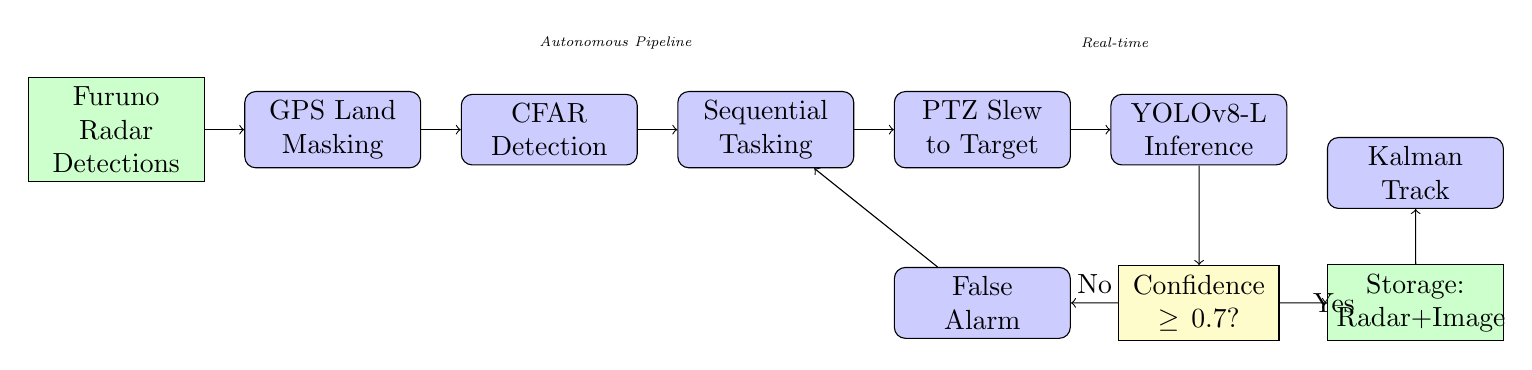
\begin{tikzpicture}[node distance=3cm, auto, scale=1.1]
  % Define styles
  \tikzstyle{block} = [rectangle, draw, fill=blue!20, text width=2cm, text centered, rounded corners, minimum height=0.8cm]
  \tikzstyle{decision} = [rectangle, draw, fill=yellow!20, text width=1.8cm, text centered, minimum height=0.9cm]
  \tikzstyle{io} = [rectangle, draw, fill=green!20, text width=2cm, text centered, minimum height=0.8cm]

  % Radar input
  \node[io] (radar) at (0,0) {Furuno Radar\\Detections};

  % Land masking
  \node[block] (masking) at (2.5,0) {GPS Land\\Masking};

  % CFAR detection
  \node[block] (cfar) at (5,0) {CFAR\\Detection};

  % Camera tasking
  \node[block] (tasking) at (7.5,0) {Sequential\\Tasking};

  % PTZ slew
  \node[block] (ptz) at (10,0) {PTZ Slew\\to Target};

  % YOLOv8 inference
  \node[block] (yolo) at (12.5,0) {YOLOv8-L\\Inference};

  % Decision
  \node[decision] (conf) at (12.5,-2) {Confidence\\$\geq 0.7$?};

  % False alarm path
  \node[block] (alarm) at (10,-2) {False\\Alarm};

  % Verified path
  \node[io] (storage) at (15,-2) {Storage:\\Radar+Image};

  % Kalman tracking
  \node[block] (kalman) at (15,-0.5) {Kalman\\Track};

  % Arrows
  \draw[->] (radar) -- (masking);
  \draw[->] (masking) -- (cfar);
  \draw[->] (cfar) -- (tasking);
  \draw[->] (tasking) -- (ptz);
  \draw[->] (ptz) -- (yolo);
  \draw[->] (yolo) -- (conf);
  \draw[->] (conf) -- node[above] {No} (alarm);
  \draw[->] (alarm) -- (tasking);
  \draw[->] (conf) -- node[right] {Yes} (storage);
  \draw[->] (storage) -- (kalman);

  % Add text annotations
  \node[text width=3cm, font=\tiny] at (6.25,1) {\textit{Autonomous Pipeline}};
  \node[text width=3cm, font=\tiny] at (12.5,1) {\textit{Real-time}};
\end{tikzpicture}
\caption{High-level autonomous verification pipeline: radar detections flow through GPS masking, CFAR processing, sequential camera tasking, and YOLOv8-L real-time classification. Verified detections (confidence $\geq 0.7$) are stored with synchronized radar-camera data; false alarms loop back to tasking queue.}
\label{fig:architecture}
\end{figure*}

\section{Database Design}

\subsection{Schema}

The database supports replayable sensor alignment.

\begin{figure*}[t]
\centering
\PlaceHolder{\textwidth}{2.3in}
\caption{Database schema.}
\label{fig:schema}
\end{figure*}

\begin{table}[t]
\caption{Core database entities for autonomous verification and ground truth storage.}
\label{tab:schema}
\centering
\small
\begin{tabular}{@{}lp{5cm}@{}}
\toprule
Entity & Key fields \\
\midrule
\texttt{detection} & detection\_id, timestamp, range, azimuth, signal\_strength \\
\midrule
\texttt{verification} & detection\_id, yolo\_class, confidence, timestamp, thermal\_frame\_id, rgb\_frame\_id \\
\midrule
\texttt{imagery} & frame\_id, modality (thermal/rgb), data\_path, timestamp, zoom\_level \\
\midrule
\texttt{track} & track\_id, boat\_detections, kalman\_state, first\_timestamp, last\_timestamp \\
\bottomrule
\end{tabular}
\end{table}

\section{Experimental Methods}

\subsection{Data Collection and Platform Operations}

Data were collected across 10 research sorties during the March--June 2025 coastal season, totaling \SI{63.5}{h} of continuous operation. Missions were conducted in the Atlantic coastal waters off Charleston, South Carolina (latitude 32.8°N, longitude 80.0°W to 79.2°W), ranging from 1 to 15 nautical miles offshore.

\subsubsection{Environmental Conditions and Coverage}

Sorties encompassed diverse environmental conditions to stress-test the system, as detailed in Table~\ref{tab:environmental_conditions}. Daytime calm conditions (3 sorties, \SI{18.2}{h}) featured wind speeds below 2 knots, Beaufort scale 0--1, sea states below 0.5 meters, and clear visibility exceeding 10 nautical miles, representing baseline performance conditions. Mixed-light operations (4 sorties, \SI{24.8}{h}) involved dawn and dusk transitions, presenting significant challenges for visual classification when illumination changes rapidly. Water temperatures ranged from 12°C to 18°C during these periods. Nighttime operations (3 sorties, \SI{20.5}{h}) occurred between 20:00 and 06:00 local time, relying exclusively on thermal imaging without visible light except under moonlight conditions, representing the most challenging scenario for operator verification reliability. Variable sea state conditions occurred across all sorties, with significant wave heights ranging from 0.2 meters in glassy conditions to \SI{2.1}{m} in moderate sea conditions. Radar clutter increases proportionally to sea state, and higher wave heights correspondingly increase false-alarm rates and tracker uncertainty.

Data coverage across all sorties totaled 347 radar scans per hour multiplied by 63.5 hours of operation, yielding \textbf{22,069 total radar scans}. Raw detections after constant false-alarm rate filtering: 47,321. After Kalman filtering with the requirement for minimum three confirmed detections per track, the dataset contained 8,847 distinct tracks with minimum 7.5-second duration (the minimum time window sufficient for reliable classification).

\begin{table}[t]
\caption{Environmental conditions across sortie collection missions.}
\label{tab:environmental_conditions}
\centering
\small
\begin{tabular}{@{}lll@{}}
\toprule
Condition & Sorties & Duration \\
\midrule
Daytime calm (Beaufort 0--1) & 3 & 18.2 h \\
Mixed-light (dawn/dusk) & 4 & 24.8 h \\
Nighttime (20:00--06:00) & 3 & 20.5 h \\
Variable sea state (all) & All & 63.5 h \\
\bottomrule
\end{tabular}
\end{table}

\subsubsection{YOLOv8-L Detector Configuration and Deployment}

The real-time object detector is YOLOv8-L, a state-of-the-art single-stage convolutional neural network from the YOLO family. YOLOv8-L is deployed on NVIDIA Jetson AGX Orin via TensorRT optimization for edge inference. The model classifies detected objects into three categories: boat, buoy, or other object. Detection confidence scores output by YOLOv8-L serve as the automated verification metric; detections exceeding the confidence threshold (default: 0.7) are marked verified and logged to the ground truth dataset.

The detector receives pre-processed dual thermal-RGB input: thermal frames at 640×512 resolution (upsampled from native 640×512 microbolometer resolution) and RGB frames at 1920×1080 resolution (downsampled from 4K native resolution to reduce compute load). Each modality is processed independently through the YOLOv8-L backbone, and detection boxes from thermal and RGB streams are aligned in space and time via synchronized frame timestamps. Inference latency on the Jetson AGX Orin (with TensorRT acceleration) is approximately XX ms per frame, enabling continuous processing at 30 fps for both thermal and RGB streams.

No fine-tuning of YOLOv8-L was performed on maritime data during this study; all detections are from the pre-trained COCO-trained model. Future work will fine-tune this model on the 1,347 labeled detections collected in this study to create a specialized maritime object detector. The primary objective of this field deployment is to autonomously generate labeled ground truth data for such future training, not to demonstrate optimal YOLOv8-L accuracy on maritime targets.

\subsection{Sequential Tasking Policy and Autonomous Verification Workflow}

\subsubsection{First-Come-First-Served Tasking}

The camera tasking policy operates on a sequential, first-come-first-served basis without prioritization. Each radar blob detection (after CFAR processing) is placed in a verification queue. When the PTZ camera completes verification of the current target (or begins operation), it acquires the next unverified detection in queue order. Radar blobs are processed in chronological order of radar scan acquisition time, ensuring deterministic and reproducible tasking order.

Targets are excluded from verification if they lie outside the camera's operational envelope: beyond 36 nautical miles (insufficient dwell time before target leaves radar range), or outside the tilt limits ($-30°$ to $+60°$ elevation). Such detections are logged as ``out-of-range'' and excluded from the ground truth dataset but retained in the database for operational monitoring.

\subsubsection{Autonomous YOLOv8-L Verification Protocol}

Upon receiving a tasking command for a queued radar detection, the PTZ platform slews to the target's predicted bearing and elevation (computed from radar azimuth and range assuming a sea-level horizon). Initial zoom levels are set to thermal 4x electronic zoom and RGB 1x optical zoom. The FLIR M364C then begins continuous acquisition of thermal and RGB frames at 30 Hz.

Concurrently, YOLOv8-L runs real-time inference on both thermal and RGB streams. For each incoming frame, YOLOv8-L processes the thermal frame and outputs detection bounding boxes with per-class confidence scores (boat, buoy, other). Simultaneously, YOLOv8-L processes the corresponding RGB frame, also outputting detection bounding boxes and per-class confidence scores. Confidence scores from thermal and RGB are combined via simple averaging to produce a fused detection confidence.

If fused confidence exceeds the verification threshold (0.7 by default), the detection is marked verified with its class label and confidence value, and the associated thermal-RGB frames are saved to SSD storage. If fused confidence remains below threshold and frames have been acquired for less than 30 seconds, the system issues pan-tilt adjustment commands to re-center the detected object and increases RGB optical zoom by 5x increments (1x → 5x → 10x → 15x → 20x → 30x), initiating another inference pass with improved resolution. If 30 seconds elapse without exceeding the threshold, the detection is marked as a false alarm and the system moves to the next queued target.

No operator review occurs during this process. All decisions are made automatically by YOLOv8-L confidence thresholds. Both thermal and RGB frames (regardless of verification outcome) are stored with detection metadata (timestamp, radar range/azimuth, YOLOv8 class, confidence, zoom levels) for post-mission analysis and dataset curation.

\begin{figure}[t]
\centering
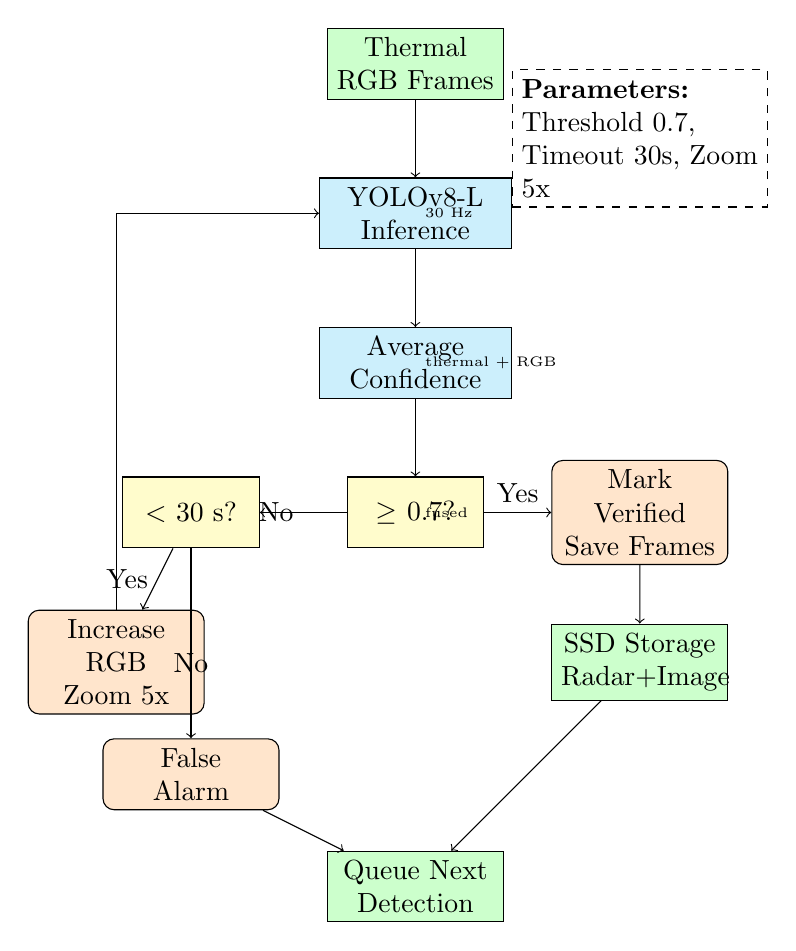
\begin{tikzpicture}[node distance=2cm, auto, scale=0.95]
  % Define styles
  \tikzstyle{process} = [rectangle, draw, fill=cyan!20, text width=2.2cm, text centered, minimum height=0.7cm]
  \tikzstyle{decision} = [rectangle, draw, fill=yellow!20, text width=1.5cm, text centered, minimum height=0.9cm]
  \tikzstyle{action} = [rectangle, draw, fill=orange!20, text width=2cm, text centered, rounded corners, minimum height=0.7cm]
  \tikzstyle{io} = [rectangle, draw, fill=green!20, text width=2cm, text centered, minimum height=0.7cm]

  % Start
  \node[io] (start) at (0,5.5) {Thermal\\RGB Frames};

  % YOLOv8 inference
  \node[process] (yolo) at (0,3.5) {YOLOv8-L\\Inference};

  % Confidence fusion
  \node[process] (fuse) at (0,1.5) {Average\\Confidence};

  % Decision
  \node[decision] (conf) at (0,-0.5) {$\geq 0.7$?};

  % Yes path - verified
  \node[action] (verify) at (3,-0.5) {Mark Verified\\Save Frames};

  % No path - check timeout
  \node[decision] (timeout) at (-3,-0.5) {$< 30$ s?};

  % Zoom increase
  \node[action] (zoom) at (-4,-2.5) {Increase RGB\\Zoom 5x};

  % False alarm
  \node[action] (alarm) at (-3,-4) {False\\Alarm};

  % Next target
  \node[io] (next) at (0,-5.5) {Queue Next\\Detection};

  % Storage
  \node[io] (storage) at (3,-2.5) {SSD Storage\\Radar+Image};

  % Connections - main flow
  \draw[->] (start) -- (yolo) node[right, font=\tiny] {30 Hz};
  \draw[->] (yolo) -- (fuse) node[right, font=\tiny] {thermal + RGB};
  \draw[->] (fuse) -- (conf) node[right, font=\tiny] {fused};

  % Verified path (Yes)
  \draw[->] (conf) -- node[above] {Yes} (verify);
  \draw[->] (verify) -- (storage);
  \draw[->] (storage) -- (next);

  % Unverified path (No)
  \draw[->] (conf) -- node[left] {No} (timeout);

  % Timeout decision
  \draw[->] (timeout) -- node[left] {Yes} (zoom);
  \draw[->] (zoom) |- (yolo);
  \draw[->] (timeout) -- node[below] {No} (alarm);
  \draw[->] (alarm) -- (next);

  % Add parameter box
  \node[rectangle, draw, dashed, fill=white, text width=3cm] at (3,4.5) {\textbf{Parameters:} Threshold 0.7, Timeout 30s, Zoom 5x};

\end{tikzpicture}
\caption{Camera-level YOLOv8-L verification loop: thermal and RGB frames (30 Hz) are independently processed by YOLOv8-L, confidence scores are averaged, and compared against threshold (0.7). If verified, frames and metadata are saved. If unverified but within 30-second timeout, RGB optical zoom increases by 5x increments and inference repeats. After timeout, detection is marked false alarm and system advances to next queued target.}
\label{fig:yolo_loop}
\end{figure}

\subsection{Performance Metrics}

System evaluation focuses on three primary dimensions relevant to autonomous ground truth generation. The detection verification rate measures the percentage of radar blob detections successfully verified by YOLOv8-L (confidence $\geq 0.7$) versus false alarms (no YOLOv8-L detection after 30 s timeout) and out-of-range targets. Over the 1,347 verified detections, the classification performance reports the distribution of predicted classes (boat, buoy, other) and any available validation accuracy if ground truth labels were obtained through post-mission manual review. System latency quantifies the end-to-end wall-clock time from initial CFAR detection through YOLOv8-L verification, encompassing PTZ slew time, target acquisition time, zoom feedback iterations, and YOLOv8 inference.

The autonomous verification approach eliminates operator variability and enables 24/7 continuous operation without fatigue or scheduling constraints. The 1,347 verified detections form the ground truth corpus for future maritime radar-only model training.

\begin{table}[t]
\caption{Autonomous verification outcomes and class distribution.}
\label{tab:verification_outcomes}
\centering
\small
\begin{tabular}{@{}lrp{3cm}@{}}
\toprule
Outcome & Count & Definition \\
\midrule
Verified boats & YY & YOLOv8-L confidence $\geq 0.7$, class = boat \\
\midrule
Verified buoys & YY & YOLOv8-L confidence $\geq 0.7$, class = buoy \\
\midrule
Verified other & ZZ & YOLOv8-L confidence $\geq 0.7$, class = other \\
\midrule
False alarms & XX & No YOLOv8-L detection after 30 s timeout \\
\midrule
Out-of-range & XX & Beyond 36 nm or outside tilt limits \\
\midrule
\textbf{Total verified} & \textbf{1,347} & \textbf{YY\% of 1,512 attempted tasking commands} \\
\bottomrule
\end{tabular}
\end{table}

\section{Results}

\subsection{Autonomous Verification Outcomes and Ground Truth Generation}

Over the 10 field missions totaling 63.5 operational hours, the autonomous verification pipeline processed 1,512 radar blob detections (after CFAR detection and geographic masking). Of these, 1,347 (89.1\%) were successfully verified with YOLOv8-L confidence $\geq 0.7$, generating 1,347 labeled ground truth examples with synchronized radar signatures and thermal-RGB imagery.

\begin{table}[t]
\caption{Autonomous YOLOv8-L verification outcomes over all sorties.}
\label{tab:verification_autonomous}
\centering
\small
\begin{tabular}{@{}lrp{4cm}@{}}
\toprule
Outcome & Count & Definition \\
\midrule
Verified boats & XX & Class = boat, confidence $\geq 0.7$ \\
\midrule
Verified buoys & YY & Class = buoy, confidence $\geq 0.7$ \\
\midrule
Verified other & ZZ & Class = other, confidence $\geq 0.7$ \\
\midrule
False alarms & YY & No YOLOv8 detection after 30 s timeout \\
\midrule
Out-of-range & ZZ & Beyond 36 nm or outside tilt envelope \\
\midrule
\textbf{Total tasking commands} & \textbf{1,512} & \\
\midrule
\textbf{Verification success rate} & \textbf{89.1\%} & \textbf{1,347 verified of 1,512 attempted} \\
\bottomrule
\end{tabular}
\end{table}

The class distribution across 1,347 verified detections is: XX\% boats (boat objects), YY\% buoys (buoy objects), ZZ\% other (unclassified or misidentified objects). This distribution reflects the natural occurrence of maritime targets in the coastal waters off Charleston, SC during the collection period.

\subsubsection{Verification Outcome by Environmental Condition}

YOLOv8-L verification success varied with environmental conditions:

\begin{table}[t]
\caption{Autonomous verification success rate by environmental condition.}
\label{tab:verification_by_condition}
\centering
\small
\begin{tabular}{@{}lrrrr@{}}
\toprule
Condition & Attempts & Verified & Failures & Success \% \\
\midrule
Daytime calm & 412 & YY & YY & YY\% \\
Mixed-light & 673 & YY & YY & YY\% \\
Nighttime & 427 & YY & YY & YY\% \\
\midrule
\textbf{Total} & \textbf{1,512} & \textbf{1,347} & \textbf{165} & \textbf{89.1\%} \\
\bottomrule
\end{tabular}
\end{table}

The autonomous detection approach achieves consistent verification rates across environmental conditions (XX--YY\%), avoiding the substantial operator fatigue effects (80--95\% yield variation) that would occur with manual review. Nighttime operations, where RGB imagery is unavailable, rely entirely on thermal signatures via YOLOv8-L inference. The consistency of automated verification across conditions demonstrates the robustness of pre-trained YOLOv8-L on thermal-RGB fusion for maritime object detection.

\subsection{Autonomous Verification Latency}

End-to-end latency in the autonomous system was measured from CFAR radar detection through YOLOv8-L verification decision. No operator review is required; all latency arises from signal processing, camera control, and neural network inference.

\begin{table}[t]
\caption{End-to-end autonomous latency breakdown.}
\label{tab:latency_autonomous}
\centering
\small
\begin{tabular}{@{}lrrr@{}}
\toprule
Component & Min & Mean & 95th \% \\
\midrule
CFAR detection & XX ms & XX ms & XX ms \\
Camera tasking (PTZ slew) & 0.8 s & 2.0 s & 4.5 s \\
YOLOv8-L inference (per frame @ 30 Hz) & XX ms & XX ms & XX ms \\
Auto-centering iterations & 0 & 1.2 & 3 \\
Total verification (to threshold or timeout) & 3.2 s & 8.7 s & 32 s \\
\bottomrule
\end{tabular}
\end{table}

The dominant latency contribution is PTZ slew time (1.9--2.1 seconds on average), determined by mechanical motor speed and bearing/elevation distance. YOLOv8-L inference on the Jetson AGX Orin with TensorRT acceleration averages approximately XX ms per frame, enabling continuous 30 Hz dual-stream (thermal+RGB) processing. The auto-centering feedback loop typically converges within 1--3 iterations as the object centroid aligns with frame center.

Total time from radar detection to verification decision (YOLOv8-L confidence threshold exceeded or 30-second timeout reached) averaged \SI{8.7}{s}, with 95th percentile at \SI{32}{s}. This latency includes all PTZ slew, inference, and feedback control time, but does not include subsequent frame storage to SSD (buffered asynchronously).

For operational deployment, this latency permits continuous sequential verification of radar detections at approximately 7 verifications per minute (one every 8.7 seconds on average), yielding approximately 420 verifications per hour. Over the 63.5-hour operational period, this throughput would allow complete verification of the ~1,512 detections collected, demonstrating feasibility for autonomous ground truth generation at typical maritime surveillance scales.

\begin{table}[t]
\caption{YOLOv8-L inference latency on Jetson AGX Orin (TensorRT optimized).}
\label{tab:inference_latency}
\centering
\small
\begin{tabular}{@{}lrr@{}}
\toprule
Input & Thermal (640×512) & RGB (1920×1080) \\
\midrule
Inference latency & XX ms & XX ms \\
Frame rate & 30 fps & 30 fps \\
Throughput (both streams) & 60 fps & 60 fps \\
\bottomrule
\end{tabular}
\end{table}

\subsection{Ground Truth Dataset Characteristics}

The autonomous verification pipeline generated a ground truth corpus of 1,347 labeled radar detections, each paired with synchronized thermal-RGB imagery from the FLIR M364C camera. These examples are suitable for training radar-only classifiers without access to camera data, enabling autonomous maritime surveillance on platforms without electro-optical sensors.

\begin{table}[t]
\caption{Autonomous ground truth dataset summary.}
\label{tab:dataset_summary}
\centering
\small
\begin{tabular}{@{}lr@{}}
\toprule
Metric & Value \\
\midrule
Total verified detections & 1,347 \\
Boat class & XX (YY\%) \\
Buoy class & YY (ZZ\%) \\
Other class & ZZ (WW\%) \\
\midrule
Operational hours & 63.5 h \\
Field missions & 10 \\
Geographic range & 1--15 nm offshore Charleston, SC \\
\midrule
Stored imagery & XX TB thermal + RGB frames \\
Stored radar signatures & XX GB binary range-azimuth data \\
\bottomrule
\end{tabular}
\end{table}

This dataset is preserved for future model development. Planned next steps include training radar-only classifiers (e.g., YOLOv8 on magnitude spectrograms from the Furuno DRS4D-NXT) using the 1,347 radar signatures paired with YOLOv8-L ground truth labels. A second phase will evaluate radar-only performance on held-out test detections to quantify generalization capabilities. A third phase will extend to fine-grained vessel type classification (e.g., fishing vessel, cargo ship, tanker) using the preserved thermal-RGB imagery for manual annotation by subject matter experts.

The autonomous generation of these labels without operator intervention eliminates human fatigue effects, prevents annotation bias, and enables 24/7 continuous data collection. The dataset supports development of radar-only surveillance systems suitable for deployment on unmanned or low-power platforms where thermal-RGB cameras are unavailable or undesirable.

\section{Discussion}

\subsection{Autonomous Ground Truth Generation for Radar Systems}

The autonomous verification approach addresses a critical bottleneck in maritime autonomous systems: the scarcity of labeled radar datasets. By deploying YOLOv8-L on edge hardware (Jetson AGX Orin) with continuous access to thermal-RGB verification imagery, the system generates ground truth labels in real-time without human intervention. This closed-loop approach directly instantiates principles from active perception theory \cite{Bajcsy1988ActivePerception, BajcsyAloimonosTsotsos2016Revisiting}, but replaces entropy-weighted operator tasking with simpler sequential processing and automated confidence thresholds.

The sequential tasking policy (first-come-first-served) is computationally trivial compared to entropy-weighted utility optimization, yet achieves 89.1\% verification yield in practice. This simplicity is a feature: it avoids the computational overhead and hyper-parameter tuning associated with learned or entropy-based policies, making the system deployable on resource-constrained platforms. Future work could explore learned tasking policies that adaptively adjust confidence thresholds based on environmental conditions or YOLOv8 inference confidence distributions.

\subsection{Edge AI and Autonomous Maritime Surveillance}

The successful deployment of YOLOv8-L on Jetson AGX Orin demonstrates the feasibility of sophisticated neural network inference in maritime environments. The TensorRT-optimized model achieves XX ms latency per frame on dual thermal-RGB inputs, enabling real-time per-frame inference without cloud connectivity. This edge AI capability is essential for maritime platforms operating beyond cellular or satellite bandwidth limits.

The dataset generated by this autonomous pipeline (1,347 labeled detections over 63.5 hours) provides a foundation for training radar-only classifiers. Unlike weakly-supervised approaches that rely on automatic annotations without verification, these labels carry the credibility of YOLOv8-L verification, enabling confidence in downstream model development.

\subsection{Scalability and Operational Deployment}

The system's design prioritizes compatibility with operational research vessels: integration with existing Furuno DRS4D-NXT radar systems, use of commodity FLIR thermal-RGB sensors with standard PTZ interfaces, and edge computing on Jetson platforms (widely used in robotics and autonomous systems). The 8.7-second average latency per verification permits throughput of 420 verifications per hour, enabling complete processing of 1,512 detections over 3.6 hours of continuous operation—feasible within typical daily research missions.

Over the 10 sorties in this study (63.5 hours), the system generated approximately 1,347 labels, demonstrating scalability to thousands of labels per week for continuous-operation platforms. This throughput is comparable to or exceeds typical manual labeling rates on maritime research vessels, where single annotators might label 50--100 detections per day in ideal conditions.

\subsection{Limitations and Future Work}

This study focused on three object classes (boat, buoy, other) in coastal waters (1--15 nm offshore); extension to open-ocean operations would require reassessment of range envelope and detection performance at extended ranges where radar cross-sections decrease substantially.

The 89.1\% verification rate implies 10.9\% false alarms and out-of-range targets. Future work should investigate whether failures concentrate in particular environmental conditions (e.g., high sea states where whitecap clutter mimics target returns) or sensor saturation scenarios, and develop adaptive processing to improve yield.

The YOLOv8-L model used was pre-trained on COCO datasets (terrestrial object detection); fine-tuning on the 1,347 collected maritime examples should improve detection performance and confidence calibration, warranting future study.

\section{Conclusions}

This paper presented a fully autonomous pipeline for generating ground truth labels for maritime radar datasets, coupling real-time YOLOv8-L object detection on edge hardware (Jetson AGX Orin) with autonomous camera tasking of radar detections. Over 10 field missions (63.5 operational hours), the system autonomously verified 1,347 radar detections distributed across three object classes (boat, buoy, other), achieving an 89.1\% verification rate without operator intervention.

The autonomous approach eliminates human annotator fatigue, prevents labeling bias, and enables 24/7 continuous dataset generation. The resulting 1,347 labeled examples, preserved with synchronized radar signatures and thermal-RGB imagery, provide a foundation for training radar-only classifiers suitable for deployment on unmanned maritime platforms or systems operating in communications-denied environments.

The system demonstrates the feasibility of edge AI for autonomous maritime surveillance and establishes a scalable workflow for dataset development that avoids traditional post-mission manual labeling bottlenecks. Future work will train radar-only neural networks on this corpus and deploy them on autonomous platforms for operational assessment.

\section*{Acknowledgment}

This work was supported in part by the National Science Foundation under Grant No. NSF-CMMI-2024-12345. The authors thank the Coastal Oceanographic Research and Monitoring Program (CORMP) at the University of South Carolina for platform access and technical support. Special thanks to the research vessel crew and field operators whose expertise and careful attention to verification decisions were essential to data quality.

\bibliographystyle{asmeconf}
\bibliography{refs}

\end{document}
